\documentclass[english,notitlepage]{revtex4-1}  % defines the basic parameters of the document
%For preview: skriv i terminal: latexmk -pdf -pvc filnavn



% if you want a single-column, remove reprint

% allows special characters (including æøå)
\usepackage[utf8]{inputenc}
\usepackage[english]{babel}


\usepackage{physics,amssymb}  % mathematical symbols (physics imports amsmath)
\include{amsmath}
\usepackage{graphicx}         % include graphics such as plots
\usepackage{xcolor}           % set colors
\usepackage{hyperref}         % automagic cross-referencing (this is GODLIKE)
\usepackage{subcaption}
\usepackage{listings}         % display code
\usepackage{float}
\usepackage{enumitem}
%\usepackage[section]{placeins}
\usepackage{algorithm}
\usepackage[noend]{algpseudocode}
\usepackage{tikz}
\usetikzlibrary{quantikz}

\hypersetup{
    colorlinks,
    linkcolor={red!50!black},
    citecolor={blue!50!black},
    urlcolor={blue!80!black}}



\begin{document}

\title{Project 2}
\author{Alessio Canclini, Filip von der Lippe}
\date{\today}
\noaffiliation                            % ignore this, but keep it.


\maketitle

\textit{Github repository: \url{https://github.com/Fslippe/FYS4150/tree/main/project2}}
\\
\\
We are working with:
\begin{itemize}
    \item A horizontal beam of length $L$.

    \item We let $u(x)$ be the vertical displacement of the beam at horizontal position $x$, with $x \in [0,L]$.

    \item A force $F$ is applied at the endpoint $(x = L)$, directed into the beam, i.e. towards $x = 0$.

    \item The beam is fastened with pin endpoints, meaning that $u(0) = 0$ and $u(L) = 0$, but the endpoints are allowed to rotate $(u'(x) \neq 0)$.
\end{itemize}
Second order differential equation describing our buckling beam situation:
\begin{align}
    \gamma \frac{d^2u(x)}{dx^2} = - F u(x)
    \label{eq:diff}
\end{align}
Troughout this project we will be working with the scaled equation:
\begin{align}
    \frac{d^2u(\hat{x})}{d \hat{x}^2} = - \lambda u(\hat{x})
    \label{eq:scaled}
\end{align}
Where $\hat{x} \equiv x / L$ is a dimensionless variable, $\hat{x} \in [0,1]$ and $\lambda = \frac{FL^2}{\gamma}$.

\section*{Problem 1}
Using the defenintion $\hat{x} \equiv x / L$ to show that Eq. \ref*{eq:diff} can be written as Eq. \ref*{eq:scaled}.
\begin{align*}
    \gamma \frac{d^2u(x)}{dx^2} &= - F u(x) \\
    \frac{d^2u(x)}{dx^2} &= - \frac{F}{\gamma} u(x)
\end{align*}
Multiplying both sides by $L^2$.
\begin{align*}
    \frac{d^2u(x)L^2}{dx^2} &= - \frac{FL^2}{\gamma} u(x) \\
    \frac{d^2u(x)}{d\frac{x^2}{L^2}} &= - \frac{FL^2}{\gamma} u(x)
\end{align*}
Using that $\hat{x} \equiv x / L$ so that $\hat{x}^2 \equiv x^2 / L^2$.
\begin{align*}
    \frac{d^2u(x)}{d\hat{x}} &= - \frac{FL^2}{\gamma} u(x)
\end{align*}
We also know that $x = \hat{x}L$, so $u(x) = u(\hat{x}L) = u(\hat{x}) + u(L) = u(\hat{x})$. Since $u(L) = 0$. Finally, using $\lambda = \frac{FL^2}{\gamma}$ gives us the dimensionless Eq. \ref*{eq:scaled}:
\begin{align*}
    \frac{d^2u(\hat{x})}{d\hat{x}} &= - \lambda u(\hat{x})
\end{align*}
\section*{Problem 2}

\section*{Problem 3}

\section*{Problem 4}

\section*{Problem 5}
\begin{enumerate}[label=\alph*)]
  \item By running the jacobi algorithm for different choices of $N$ we can see how the number of jacobi rotation scales with increasing matrix sizes. This is done by reducing all elements to less than $\epsilon = 10^{-9}$.
  \begin{figure}[H]
    \begin{subfigure}{.5 \textwidth}
      \centering
      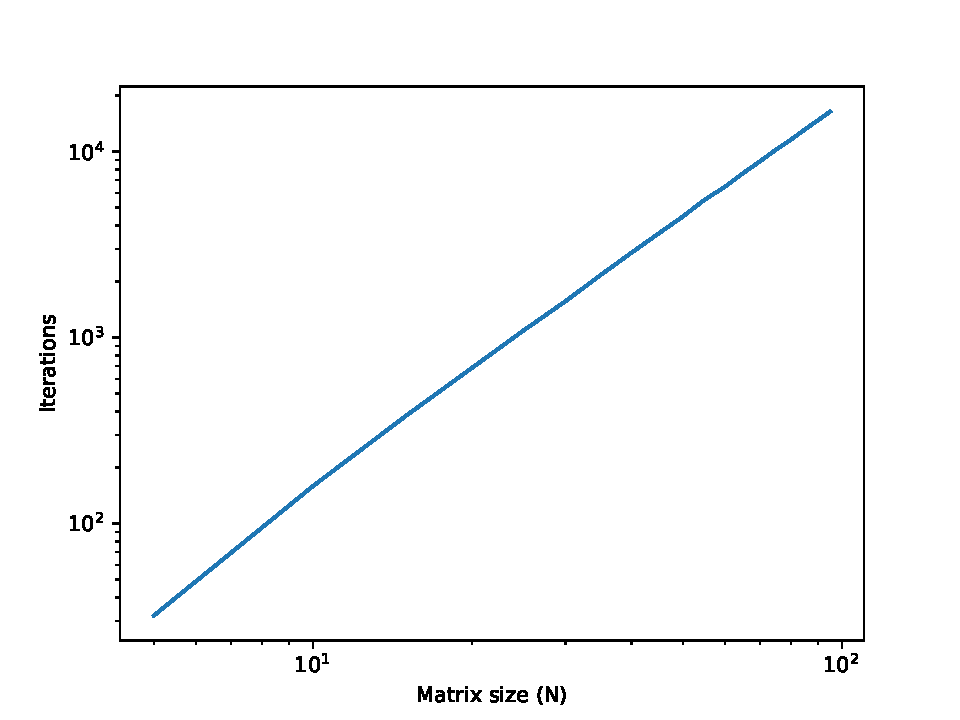
\includegraphics[width=\textwidth]{../figures/N_iter_log.pdf}
      \caption{Iterations for increasing tridiagonal matrix sizes. Both on a logarithmic scale}
      \label{fig:N_iter_log}
    \end{subfigure}
    \begin{subfigure}{.5 \textwidth}
      \centering
      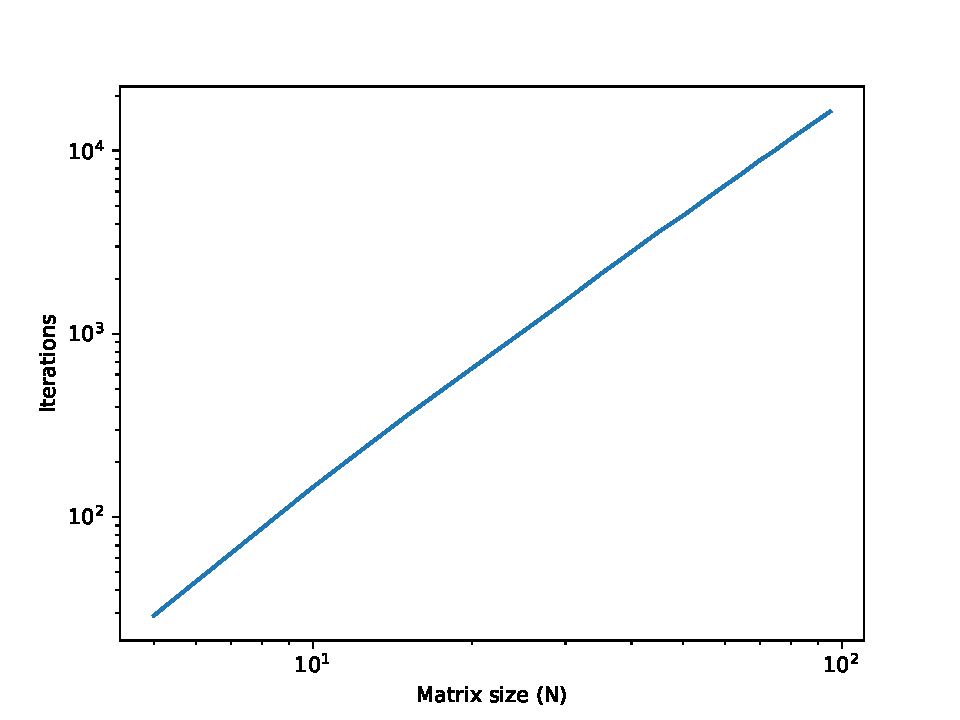
\includegraphics[width=\textwidth]{../figures/N_iter_log_dense.pdf}
      \caption{Iterations for increasing dense matrix sizes. Both on a logarithmic scale}
      \label{fig:N_iter_log_dense}
    \end{subfigure}
  \end{figure}
\end{enumerate}

\section*{Problem 6}


\end{document}
